\newcommand\tab[1][1cm]{\hspace*{#1}}
\section{Netzwerkverbindungen (ES)}
\subsection{TCP}
\subsubsection{Definition}
''Das Transmission Control Protocol (TCP) ist ein zuverlässiges, verbindungsorientiertes, Bytestrom Protokoll. Die Hauptaufgabe von TCP besteht in der Bereitstellung eines sicheren Transports von Daten durch das Netzwerk. TCP ist im RFC 793 definiert. Diese Definitionen wurden im Laufe der Zeit von Fehlern und Inkonsistenzen befreit (RFC 1122) und um einige Anforderungen ergänzt (RFC 1323). Das Transmission Control Protocol stellt die Zuverlässigkeit der Datenübertragung mit einem Mechanismus, der als Positive Acknowledgement with Re-Transmission (PAR) bezeichnet wird, bereit. Dies bedeutet nichts anderes als das, daß das System, welches Daten sendet, die Übertragung der Daten solange wiederholt, bis vom Empfänger der Erhalt der Daten quittiert bzw. positiv bestätigt wird. Die Dateneinheiten, die zwischen den sendenden und empfangenden TCP-Einheiten ausgetauscht werden, heißen Segmente. Ein TCP-Segment besteht aus einem mindestens 20 Byte großen Protokollkopf und den zu übertragenden Daten. In jedem dieser Segmente ist eine Prüfsumme enthalten, anhand derer der Empfänger prüfen kann, ob die Daten fehlerfrei sind. Im Falle einer fehlerfreien Übertragung sendet der Empfänger eine Empfangsbestätigung an den Sender. Andernfalls wird das Datengramm verworfen und keine Empfangsbestätigung verschickt. Ist nach einer bestimmten Zeitperiode (timeout-period) beim Sender keine Empfangsbestätigung eingetroffen, verschickt der Sender das betreffende Segment erneut.'' \cite{noauthor_einfuhrung_nodate}
\subsubsection{Verifizierung}
''TCP ist ein verbindungsorientiertes Protokoll. Verbindungen werden über ein Dreiwege-Handshake (three-way handshake) aufgebaut. Über das Dreiwege-Handshake werden Steuerinformationen ausgetauscht, die die logische Ende-zu-Ende-Verbindung etablieren. Zum Aufbau einer Verbindung sendet ein Host (Host 1) einem anderen Host (Host 2), mit dem er eine Verbindung aufbauen will, ein Segment, in dem das SYN-Flag gesetzt ist. Mit diesem Segment teilt Host 1 Host 2 mit, das der Aufbau einer Verbindung gewünscht wird. Die Sequenznummer des von Host 1 gesendeten Segments gibt Host 2 außerdem an, welche Sequenznummer Host 1 zur Datenübertragung verwendet. Sequenznummern sind notwendig, um sicherzustellen, daß die Daten vom Sender in der richtigen Reihenfolge beim Empfänger ankommen. Der empfangende Host 2 kann die Verbindung nun annehmen oder ablehnen. Nimmt er die Verbindung an, wird ein Bestätigungssegment gesendet. In diesem Segment sind das SYN-Bit und das ACK-Bit gesetzt. Im Feld für die Quittungsnummer bestätigt Host 2 die Sequenznummer von Host 1, dadurch, daß die um Eins erhöhte Sequenznummer von Host 1 gesendet wird. Die Sequenznummer des Bestätigungssegments von Host 2 an Host 1 informiert Host 1 darüber, mit welcher Sequenznummer beginnend Host 2 die Daten empfängt. Schlußendlich bestätigt Host 1 den Empfang des Bestätigungssegments von Host 2 mit einem Segment, in dem das ACK-Flag gesetzt ist und die um Eins erhöhte Sequenznummer von Host 2 im Quittungsnummernfeld eingetragen ist. Mit diesem Segment können auch gleichzeitig die ersten Daten an Host 2 übertragen werden. Nach dem Austausch dieser Informationen hat Host 1 die Bestätigung, daß Host 2 bereit ist Daten zu empfangen. Die Datenübertragung kann nun stattfinden. Eine TCP-Verbindung besteht immer aus genau zwei Endpunkten (Punkt-zu-Punkt-Verbindung).'' \cite{noauthor_einfuhrung_nodate}
\begin{figure}
\begin{center}
    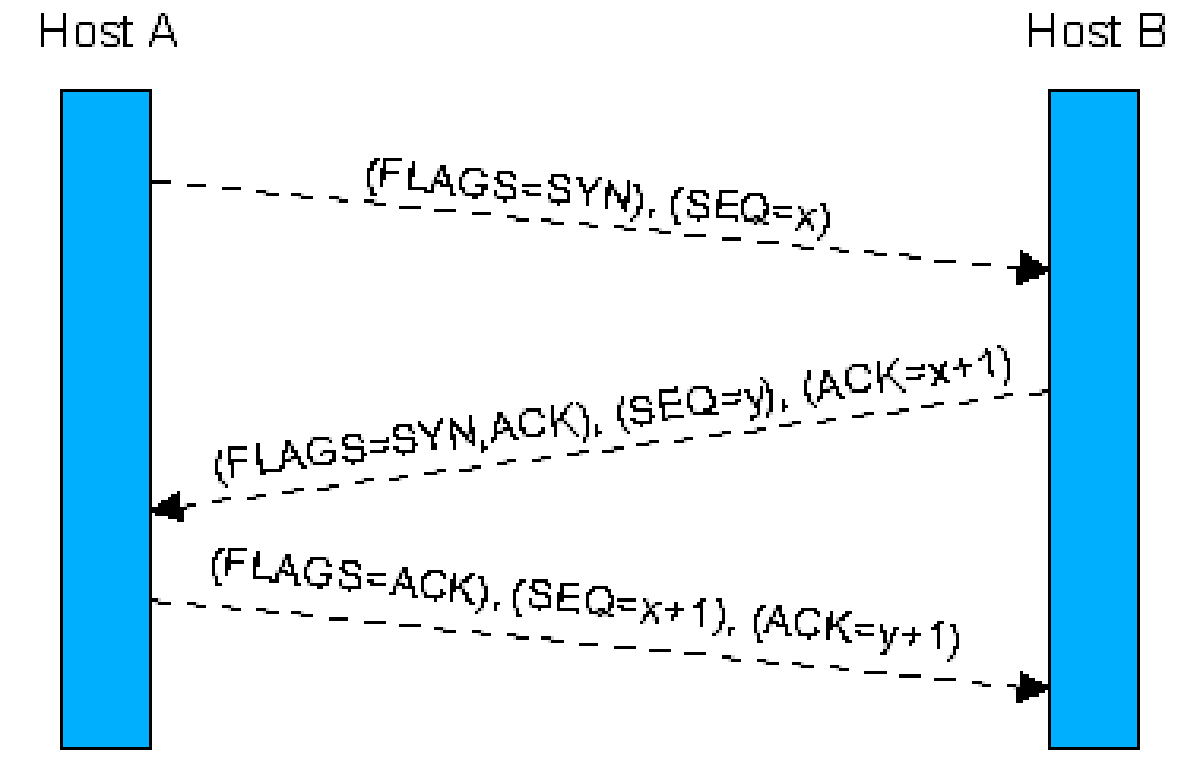
\includegraphics[scale=0.35]{images/ThreeWayHandshake.png} 
\end{center}
    \caption{three-way handshake \cite{noauthor_einfuhrung_nodate}}
    \label{img:three-way handshake}
    
\end{figure}
\subsection{TCP-Client} \label{TCP-Client} %Schreibweise ?
\subsubsection{Übersicht}
Der TCP-Client stellt Clientverbindungen für TCP-Netzwerkdienste bereit. Die TCP-Client Klasse bietet einfache Methoden zum Herstellen einer Verbindung, senden und empfangen von Daten. Der TCP-Client verbindet sich mit einem TCP-Listener und stellt danach einen Network Stream zur Verfügung, welcher ausgelesen werden kann und auf welchem geschrieben werden kann. Zum Verbinden mit einem TCP-Listener gibt es zwei Möglichkeiten:
Der TCP-Client stellt “Connect” Methoden zur Verfügung, oder man kann im Konstruktor bereits die IP-Adresse und den Port angeben. Im Konstruktor wird dann die Verbindung automatisch hergestellt.
Wenn die Verbindung besteht, kann mit .GetStream() der Network Stream des TCP-Clients abrufen und diesen mit .Read(Byte[],Int32,Int32) auslesen oder diesen mit .Write(Byte[],Int32,Int32) beschreiben. Wenn der Kommunikationsaustausch abgeschlossen ist, sollte der TCP-Client mit .Close(Int32) geschlossen werden.
\subsubsection{Konstruktoren}
Name: \textbf{TCPClient()}
\newline
Info: Erstellt einen TCP-Client, der noch zu keinem TCP-Listener verbunden ist.
\newline
\newline
Name: \textbf{TCPClient(IPEndpoint)}
\newline
Info: Erstellt einen TCP-Client, welcher sich im Konstruktor bereits zu dem angegebenen IPEndpoint verbindet.
\newline
\newline
Name: \textbf{TCPClient(string, Int32)}
\newline
Info: Erstellt einen TCP-Client, welcher sich im Konstruktor bereits zu der als String angegebenen IP-Adresse und dem als Int32 angegebenen Port verbindet.
\subsubsection{Methoden}
Name: \textbf{Close()}
\newline
Info: Schließt die Verbindung zum Remotehost.
\newline
\newline
Name: \textbf{Connect()}
\newline
Info: Verbindet den TCP-Client mit dem Remotehost. Dazu gibt es verschiedene Parameter:
\newline \tab \newline
- \textit{Connect(IPAdress, Int32)}, wobei hier die IP-Adresse bereits als IPAdress-Objekt und der Port als Int32 mitgegeben wird.
\newline \tab \newline
- \textit{Connect(IPAdress[], Int32)} wird benutzt wenn der Remotehost mehrere DNS-Einträge hat und man nicht genau weiß, welcher der richtige ist. Es wird eine Liste aller IP-Adressen mitgegeben, wobei es sich auch hier um IPAdress-Objekte handelt. Auch hier wird der Port als zweiter Parameter als Int32 mitgegeben.
\newline \tab \newline
- \textit{Connect(IPEndPoint)}: Hier wird direkt ein IPEndPoint-Objekt mitgegeben, welches bereits alle relevanten Infos über den Remotehost beinhaltet.
\newline \tab \newline
- \textit{Connect(string, Int32)}: Die einfachste Methode, da hier die IP-Adresse einfach als String mitgegeben wird. Auch hier wird als zweiter Parameter der Port als Int32 angegeben.
\newline
\newline
Name: \textbf{ConnectAsync()}
\newline
Info: Verbindet den TCP-Client mit dem Remotehost asynchron. Dazu gibt es verschiedene Parameter:
\newline \tab \newline
- \textit{ConnectAsync(IPAdress, Int32)}, wobei hier die IP-Adresse bereits als IPAdress-Objekt und der Port als Int32 mitgegeben wird.
\newline \tab \newline
- \textit{ConnectAsync(IPAdress[], Int32)} wird benutzt wenn der Remotehost mehrere DNS-Einträge hat und man nicht genau weiß welcher der richtige ist. Es wird eine Liste aller IP-Adressen mitgegeben, wobei es sich auch hier um IPAdress-Objekte handelt. Auch hier wird der Port als zweiter Parameter als Int32 mitgegeben.
\newline \tab \newline
- \textit{ConnectAsync(string, Int32)}: Die einfachste Methode, da hier die IP-Adresse einfach als String mitgegeben wird. Auch hier wird als zweiter Parameter der Port als Int32 angegeben.
\newline \newline
Name: \textbf{Dispose()}
\newline
Info: Gibt alle vom TCP-Client verwendeten Ressourcen frei.
\newline \newline
Name: \textbf{GetStream()}
\newline
Info: Gibt den Network Stream zurück, welcher für das Senden und Empfangen von Daten wichtig ist.
\newline
\subsubsection{Verwendung in Ludimus}
Die Verbindung zwischen Smartphone und Server(PC/Laptop) baut auf einem Network Stream auf, also ist es notwendig die Verbindung per TCP-Client und TCP-Listener durchzuführen. Zusätzlich bietet TCP, hier viele Vorteile weshalb die Wahl zum TCP-Client nicht schwer fiel. In Ludimus ist jedes Smartphone, welches sich mit dem Server, per TCP-Verbindung, verbindet, ein TCP-Client, welcher in einer Liste gespeichert wird und so für jeden zur Verfügung stehen. Zusätzlich gibt es die .SendData(string key,string value) Methode welche den Zugriff auf den Network Stream über den TCP-Client löst.
\subsection{TCP-Listener} \label{TCP-Listener}
\subsubsection{Übersicht}
Die TCP-Listener Klasse bietet einfache Methoden, die das akzeptieren von eingehenden Verbindungsanfragen erlauben. Die TCP-Listener Klasse wird zusammen mit dem TCP-Client benutzt, um eine Verbindung miteinander aufzubauen und per Network Stream zu kommunizieren. Dem TCP-Listener selbst wird dabei im Konstruktor als Parameter die IP-Adresse und der Port, auf welchem der TCP-Listener hören soll, mitgegeben. Als IP-Adresse kann auch Any mitgegeben werden, um den TCP-Listener auf der lokalen IP-Adresse laufen zu lassen. Um den TCP-Listener zu starten, muss einfach .Start() aufgerufen werden und somit horcht der TCP-Listener auf der angegeben IP-Adresse und Port. Eingehende Verbindungsanfragen werden in eine Warteschlange gereiht. Mit .AcceptSocket() oder .AcceptTCP-Client() wird die erste Verbindungsanfrage aus der Warteschlange genommen und kann dann an einen TCP-Client weitergegeben werden. Die .AcceptSocket() und .AcceptTCP-Client() Methoden blockieren jedoch und warten bis auch wirklich eine Verbindungsanfrage kommt. Diese beiden Methoden in einen Thread auslagern macht durchaus Sinn. Wenn man jedoch keinen Thread benutzen will, kann man auch einfach mit der .Pending() Methode abfragen, ob in der Warteschlange eine Verbindungsanfrage eingereiht ist. Mit der .Stop() Methode kann der TCP-Listener gestoppt werden. Die .Stop() Methode jedoch schließt nicht alle vorhandenen TCP-Client Verbindungen. Diese danach noch sauber zu schließen liegt in der Hand des Programmierers.
\subsubsection{Konstruktoren}
Name: \textbf{TCPListener(Int32)}
\newline
Info: Erstellt einen TCP-Listener, welcher auf dem als Int32 angegebenen Port horcht.
\newline \newline
Name: \textbf{TCPListener(IPAdress, Int32)}
\newline
Info:  Erstellt einen TCP-Listener, welcher auf der lokalen, als IPAdress Objekt übergebenen IP-Adresse und dem als Int32 angegebenen Port horcht.
\newline \newline
Name: \textbf{TCPListener(IPEndpoint)}
\newline
Info: Erstellt einen TCP-Listener, welcher auf dem angegebenen IPEndpoint horcht.
\newline \newline
\subsubsection{Methoden}
Name: \textbf{AcceptSocket()}
\newline
Info: Gibt den ersten Socket in der Request-Warteschlange zurück. Blockiert den Thread, in welchem die Methode aufgerufen wurde.
\newline \newline
Name: \textbf{AcceptSocketAsync()}
\newline
Info: Gibt den ersten Socket in der Request-Warteschlange zurück. Wird asynchron ausgeführt.
\newline \newline
Name: \textbf{AcceptTCPClient()}
\newline
Info: Gibt den ersten TCP-Client in der Request-Warteschlange zurück. Blockiert den Thread, in welchem die Methode aufgerufen wurde.
\newline \newline
Name: \textbf{AcceptTCPClientAsnyc()}
\newline
Info: Gibt den ersten TCP-Client in der Request-Warteschlange zurück. Wird asynchron ausgeführt.
\newline \newline
Name: \textbf{Start()}
\newline
Info: Der TCP-Listener startet und wartet ab jetzt auf eingehende Verbindungsanfragen.
\newline \newline
Name: \textbf{Stop()}
\newline
Info: Der TCP-Listener stoppt und horcht nicht mehr auf eingehende Verbindungsanfragen. Wichtig: Durch Stop werden die TCP-Client Verbindungen nicht sauber geschlossen.
\newline \newline
\subsubsection{Implementierung in Ludimus}
Beim Starten der PC/Laptop App wird ein TCP-Listener gestartet, welcher auf die eingehenden Verbindungsanfragen der Smartphones, auf welchen ein TCP-Client läuft, horcht. Der TCP-Listener nimmt maximal acht Verbindungen an. Er wird in einem extra Thread geöffnet, welcher permanent im Hintergrund läuft. Somit wird, bis acht Verbindungen erreicht wurden, permanent auf Verbindungsanfragen geachtet. Wenn eine Verbindungsanfrage ankommt wird sie mit hilfe der .AcceptTCP-Client() Methode angenommen und einem Player-Objekt übergeben.
\subsection{Network Streams} \label{ns}
\subsubsection{Übersicht}
Network Ressourcen werden im .Net Framework als Streams angesehen, diese heißen Network Streams. Eigenschaften von Network Streams sind unter anderem, dass egal welchen Datentyp sie senden oder lesen, dies mit den .Write() und .Read() Methoden möglich ist. Außerdem sind sie sehr ähnlich den anderen im .Net Framework oft benutzten Streams. Der einzige Unterschied ist, dass die Network Streams nicht suchbar sind. Die .Seek() und .Position() Methoden werfen bei Network Streams eine NotSupportedException. Network Streams sind ein Teil des System.Net.Sockets Namespaces. Die Network Stream Klasse bietet Methoden für das Senden und Empfangen von Daten, dabei hat die Network Stream Klasse Methoden für asynchrones und synchrones Senden und Empfangen. Um einen Network Stream zu bekommen muss bereits vorher eine Socket oder TCP Verbindung zwischen den beiden kommunizierenden Geräten vorhanden sein. Zu beachten ist, dass wenn man den Network Stream schließt nicht automatisch auch die Socket oder TCP Verbindung geschlossen wird, sondern der Programmierer diese noch extra sauber schließen muss. Um das ganze synchron zu machen, reichen die oben bereits angesprochenen .Write() und .Read() Methoden, die allerdings den jeweiligen Thread blockieren. Um das ganze asynchron zu machen, sollte man die .BeginRead()/.EndRead() und .BeginWrite()/.EndWrite Methoden benutzen. Diese geben ein IAsyncResult zurück und sind damit dafür besser geeignet. Solange man jedoch einen eigenen Thread für die .Write() und für die .Read() Methode hat können beide synchron auf dem Network Stream eingesetzt werden.
\subsubsection{Methoden}
Name: \textbf{Close(Int32)}
\newline
Info: Schließt den Network Stream nach einer, durch Parameter angegebenen, Zeit in welcher noch Daten über den Network Stream gesendet werden.
\newline \newline
Name: \textbf{CopyTo(Stream,Int32)}
\newline
Info: Kopiert den gesamten Network Stream in einen anderen Stream, welcher durch die Parameter angegeben wird. Zusätzlich kann, in Form eines Int32, auch eine Buffergröße angegeben werden, diese dient zur Beschränkung des kopierten Bereichs.
\newline \newline
Name: \textbf{Dispose()}
\newline
Info: Gibt alle vom Network Stream benutzten Methoden frei.
\newline \newline
Name: \textbf{Flush()}
\newline
Info: Löscht die kompletten Daten des Streams.
\newline \newline
Name: \textbf{Read(Byte[],Int32,Int32)}
\newline
Info: Liest den Network Stream aus. Das Byte Array gibt dabei den Buffer an, in welchem die empfangenen Daten geschrieben werden. Der zweite Parameter an welcher Stelle angefangen wird in den Buffer zu schreiben und der dritte Parameter legt fest wie viel eingelesen werden soll.
\newline \newline
Name: \textbf{Write(Byte[],Int32,Int32)}
\newline
Info: Schreibt in den Network Stream. Das Byte Array gibt dabei den Buffer an, der die Daten gespeichtert hat, die versendet werden sollen. Der zweite Parameter an welcher Stelle des Buffers angefangen wird zu senden und der dritte Parameter legt fest wie viel vom Buffer versendet werden soll.
\newline \newline